\section{Peeragogy}\label{sec:Peeragogy} 
%% Possibly change to Peeragogy in Action.
%% Maybe change Wrapper to Wrap Up, or call the other patterns according to roles
% DK: I question whether the Peeragogy Project is a pattern, or an instance of a pattern. We generally think about patterns as something that can be instantiated. But your project seems like a specific case of the concept.
% JC: There could be many projects

\subsubsection*{Motivation} This pattern is relevant to anyone who wants to do active learning together with others in a relatively non-hierarchical setting.

\subsubsection*{Context} Collaborative projects like Wikipedia, StackExchange, and FLOSS represent an implicit challenge to the old ``industrial'' organization of work.  This new way of working appears to promise something more resilient, more exciting, and more humane.  The rhetoric has been questioned \cite{shawlaboratories,kreiss2011limits}; but it is clear that in the context of these ``free'', ``open'', post-modern organizations, individual participants are learning \cite{schmidt+commons-based+2009} -- and that they collectively adapt the methods and infrastructure as they go.
Because everyone in these projects primarily learns by putting in effort on a shared work-in-progress, participants are more in touch with an \emph{equality of intelligence} than an \emph{inequality of knowledge} \cite[pp.~38, 119]{ranciere1991ignorant}.
At the same time, they invoke a form of friendly competition, in which \emph{the best craftmanship wins} \cite[p.~89]{raymond2001cathedral}.
%%% FORCES

\subsubsection*{Forces}~
\begin{tabular}[t]{p{.8\textwidth}@{\hspace{.03\textwidth}}c}
\textbf{Threshold}: inclusiveness and specificity are in tension. & {\icon \symbol{"00220A}} \\
\textbf{Trust}: is only built through sharing and reciprocity. & {\icon \symbol{"002158}}
\\
\end{tabular}

\subsubsection*{Problem} Even a highly successful project like Wikipedia is a work in progress that can be improved to \emph{\emph{better} empower and engage people around the world, to develop \emph{richer and more useful} educational content, and to disseminate it \emph{more} effectively} -- and deploy it more creatively.\footnote{\url{https://wikimediafoundation.org/wiki/Mission_statement}}  How to go about this is a difficult question, and we don't know the answers in advance.  There are rigorous challenges facing smaller projects as well, and fewer resources to draw on.  Many successful free software projects are not particularly collaborative -- and the largest projects are edited only by a small minority of users \cite{free-software-better,who-writes-wikipedia}.  Can we work smarter together?

\subsubsection*{Solution} The act of asking ``can we work smarter together?'' puts learning front and center.  Peeragogy takes that ``center'' and distributes it across a pool of heterogeneous relationships.  Indeed, peeragogy can be understood as an up-to-date revision of Alexander's \patternnameext{Network of Learning} \cite[p. 99]{alexander1977pattern}.  It \emph{decentralizes the process of learning and enriches it through contact with many places and people} in interconnected networks that may reach all over the world.   Importantly, while people involved in a peeragogical process may be collaborating on \patternname{A specific project}, they don't have to be direct collaborators outside of the learning context or co-located in time or space.  Just as theories and practices of pedagogy articulate the transmission of knowledge from teachers to students, peeragogy articulates the way peers produce and use knowledge together (Figure \ref{fig:connections}).
% Can we clarify that we're describing Peeragogy as a pattern, and a pattern language, and that it is useful whether or not others decide to use patterns...
%OSS: We talk about patterns - does this mean learners are meant to organize their knowledge in new patterns? Would be great if learners made new patters, but we're not requiring that and we need to be more explicit about that? May also be useful for people into pattersns


\subsubsection*{Rationale}
% DK: I have written many, and shepherded many more, and I don’t think this is the case. However, the effort that goes into writing them makes them more intuitive to read :+)
The peeragogical approach particularly addresses the problems of small projects stuck in their individual silos, and large projects becoming overwhelmed by their own complexity.  It does this by going the opposite route: explicating \emph{what by definition is tacit} and employing \emph{a continuous design process} \cite[pp. 9--10]{schummer2014beyond}.   Active learning together with others brings social and emotional intelligence to bear on the things that matter most.

\subsubsection*{Resolution}

Peeragogy helps people in different projects describe and solve real problems. 
If you share the problems that you're experiencing with others, there's a reasonable chance that someone may be able to help you solve them.  Bringing a problem across the \textbf{threshold} of someone else's awareness helps achieve clarity.  
This process can guide individual action in ways that we wouldn't have seen on our own, and may lead to new forms of collective action we would never have imagined possible.  People who gain experience comprehending problems together build \textbf{trust}.
%
Making room for multiple right answers contributes further to resolving the tension between generality and specificity.

%% \subsubsection*{Inversion}
%% Celebrated mathematician Michael Atiyah points out that, the benefits
%% of collaboration notwithstanding, ``many mathematicians do not like or
%% are incapable of collaborating with other mathematicians,'' and he
%% further remarks that ``when it comes to the crunch, there is no
%% substitute for really hard thinking on your own''
%% \cite{atiyah1974research}.  Don't use \patternname{Peeragogy}, or use
%% it in limited forms, if the cost of building trust is prohibitive, or
%% when sharing your concerns with others brings no advantage.


\subsubsection*{Example 1} Wikipedia and its sister sites Wiktionary, Wikiversity, etc. (collectively ``Wikimedia'') rely on user-generated content,
peer produced software, and are managed, by and large, by a pool of users who choose to
get involved with governance and other ``meta'' duties.\footnote{\url{https://www.wikimedia.org/}}
%
The Wikimedia Foundation maintains the servers and acts on behalf of
this ``global movement''.  They achieve something quite impressive:
Wikipedia is the 7\textsuperscript{th} most popular website in the
world, but the Wikimedia Foundation has under 300 employees.  For
comparison, the 6\textsuperscript{th} (Amazon) and
8\textsuperscript{th} (QQ) most popular websites are run by companies
with over 200K and 28K employees,
respectively.\footnote{\url{https://en.wikipedia.org/wiki/Wikimedia_Foundation\#Employees}}\textsuperscript{,}\footnote{\url{http://phx.corporate-ir.net/phoenix.zhtml?c=97664&p=irol-newsArticle&ID=2100418}}\textsuperscript{,}\footnote{\url{https://www.google.com/finance?cid=695431}}\textsuperscript{,}\footnote{\url{http://www.alexa.com/topsites}}
%OSS: which ones are they?   


\begin{wrapfigure}{r}{.48\textwidth}
\vspace{-.65cm}
\begin{center}
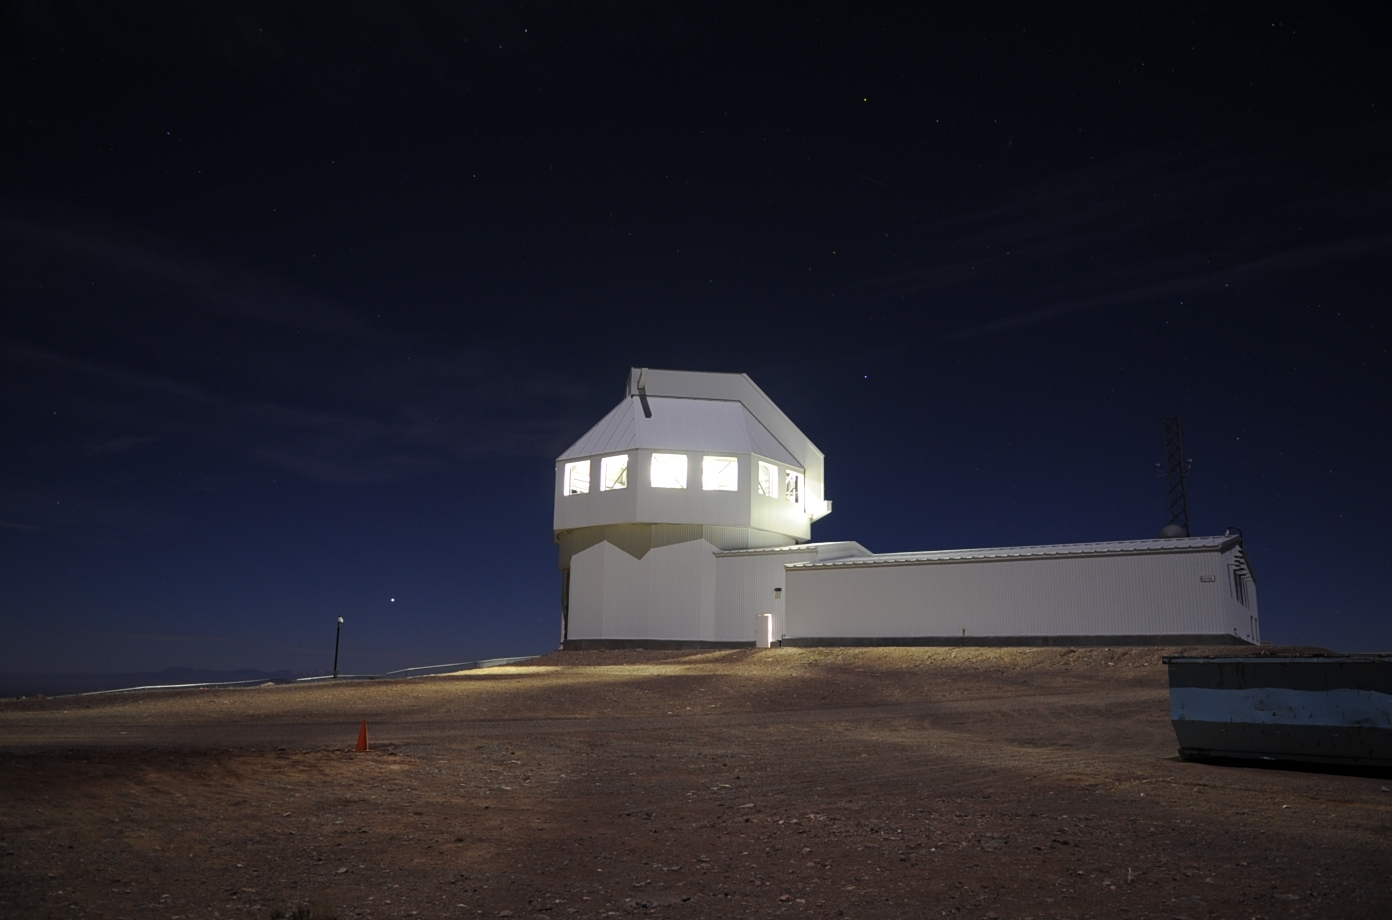
\includegraphics[width=.48\textwidth,trim=0 170 0 250, clip=true]{Space_Surveillance_Telescope}
\end{center}
\vspace{-.5cm}
\captionsetup{font=footnotesize,width=.48\textwidth}
\caption{\textsl{Observatory}: Space Surveillance Telescope, New Mexico.
%Public domain.
\label{space-surveillance}}
\vspace{-1.1cm}
\end{wrapfigure}

\subsubsection*{Example 2} Although one of the strengths of \patternname{Peeragogy} is to
distribute the workload, this does not mean that infrastructure is
irrelevant.  The students and
researchers of the future university will need access to an
Observatory and other scientific apparatus if they are to
reach \emph{ad astra, per aspera} (Figure \ref{space-surveillance}).\footnote{Latin: ``With difficulty, to the stars.''}

\smallskip

\begin{framed}
\noindent 
\emph{What's Next in the Peeragogy Project}
\definecollection{PeeragogyWN}
\begin{collectinmacro}{\PeeragogyWN}{}{}
We intend to revise and extend the \emph{Patterns of Peeragogy} into a framework that can describe and scaffold the learning that happens inside and outside of institutions.
\end{collectinmacro}
\PeeragogyWN
\end{framed}

% People won't get invested without a return, although this may not be the same for everyone.
% , and the idea of a specific goal or something concrete on offer
